\documentclass[sigconf,screen]{cidr-2027}

\usepackage{amsmath}
\usepackage{array}
\usepackage{booktabs}
\usepackage{graphicx}
\usepackage{xspace}

\graphicspath{{../images/}}
\settopmatter{printccs=false, printacmref=false}
\setlength{\emergencystretch}{2em}

\newcommand{\sys}{SemL0\xspace}
\newcommand{\exact}{\textsc{Exact}\xspace}
\newcommand{\cons}{\textsc{Conservative}\xspace}
\newcommand{\unknown}{\textsc{Unknown}\xspace}

\title{\sys: Query Signatures for Dynamic Property-Graph Storage}

% CIDR is single-blind. The paper owner must replace these placeholders.
\author{Author Name(s)}
\affiliation{%
  \institution{Institution}
  \country{Country}
}
\email{email@example.com}

\begin{abstract}
Typed-neighbor reads already reveal source labels, edge types, direction, and
other graph semantics, yet LSM storage usually admits files and schedules
compaction using only keys, levels, and bytes. This mismatch creates semantic
read amplification and lets compaction erase metadata that once proved a file
irrelevant. We present \sys, a lifecycle-oriented prototype in which query
signatures become persistent storage-admission evidence. Its contract permits
skipping under exact evidence or a safe conservative over-approximation, but
never under unknown evidence. A file budget selects which label/type groups
receive degree-exact L0 partitions;
unselected groups retain schema-level pruning.

Stage-specific experiments on LDBC SNB data show the tradeoff. At SF10,
budget-64 uses 13.3~GiB, 444 L0 files, and 2.26~GiB peak import RSS, versus
14.6~GiB, 737 files, and 8.38~GiB for full semantic materialization. At SF100,
the corresponding RSS values are 2.21 and 118.03~GiB. Controlled compaction
and a real 1.09-billion-edge SF30 run show that semantic merge retains the
pruning surface, while naive merge destroys it; the SF30 read consequence is a
metadata-replay proxy, not a full body-read speedup. The evidence is decomposed
by lifecycle stage rather than claimed as one end-to-end validation.
\end{abstract}

\ccsdesc[500]{Information systems~Graph-based database models}
\ccsdesc[300]{Information systems~Data structures}
\ccsdesc[300]{Information systems~Storage management}

\keywords{dynamic graphs, LSM-tree, property graph, storage layout, compaction}

\begin{document}
\maketitle

\section{Motivation and Thesis}

Property-graph reads ask for semantic neighborhoods, for example outgoing
\texttt{KNOWS} edges from a \texttt{Person}, rather than an undifferentiated
key range. LDBC SNB makes typed neighborhoods central to its workload
\cite{ldbc}. Dynamic graph stores nevertheless benefit from LSM organization:
updates enter a mutable component, flush into immutable segments, and are
rewritten by compaction \cite{lsm,lsmgraph}. The problem is that a selective
query may know its edge type while storage metadata cannot prove that most L0
segments are irrelevant. It must then admit and inspect them.

Compaction makes this more than a query-time filtering problem. Suppose three
segments represent Person acquaintances, Person-to-post likes, and Forum
membership as separate exact partitions. A naive merge can preserve every
logical edge while emitting a mixed segment. Future queries lose the proof
required to skip unrelated bytes. Thus, compaction is not semantically neutral:
it changes the future pruning surface.

\sys studies the thesis that query semantics should be a \emph{budgeted
storage control plane}. The implementation contributes: (1) a storage
signature and an explicit safe-skip contract; (2) a budget algorithm that
interpolates between a strong schema layout and full semantic materialization;
and (3) semantic-aware compaction that preserves or rebuilds useful evidence.
We claim a \emph{lifecycle-oriented design with stage-specific evidence}, not
one experiment that validates the complete lifecycle. The current property
support is also deliberately narrow: storage admission summarizes property
presence, not arbitrary equality, range, or \texttt{WHERE} predicates.

This framing produces three concrete systems questions. First, what semantic
state can an immutable segment expose without making correctness depend on an
optional index? Second, where should a finite file budget be spent when the
schema layout already provides useful label/type pruning? Third, how can a
rewrite retain that state without turning every compaction into full semantic
repartitioning? We answer these questions with the following contributions:

\begin{itemize}
\item We define a storage-admission interface that separates a query's
semantic signature from MVCC visibility and schema resolution. Its
\exact/\cons/\unknown contract makes each skipped segment a proof obligation.
\item We implement a file-budgeted L0 layout. It ranks source-label/edge-type
groups by configured or observed demand, charges the estimated number of
degree-exact files, and leaves unselected groups at the schema baseline.
\item We make semantic-surface retention an explicit compaction objective and
measure its read/write consequence on controlled inputs and real SF30
metadata, while reporting the limits of each experiment.
\end{itemize}

\section{Design}

\begin{figure*}[t]
  \centering
  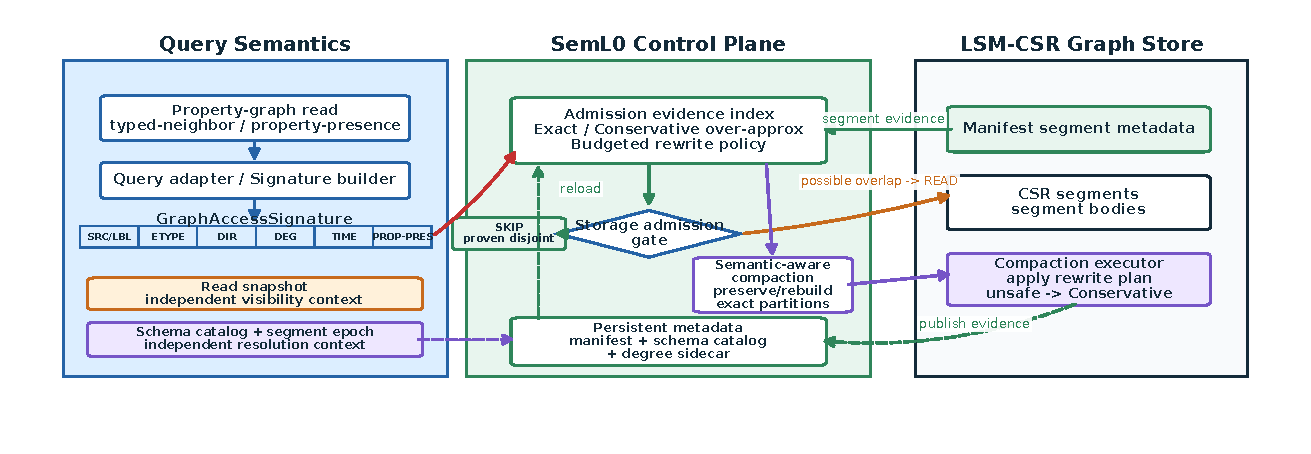
\includegraphics[width=0.98\textwidth]{fig1_system_control_plane.pdf}
  \caption{The \sys control plane, aligned with the implementation. A
  \texttt{GraphAccessSignature} contains storage-admission facts; the read
  snapshot and schema/segment-epoch resolution are independent contexts.
  Exact disjointness, proven absence, or disjoint conservative
  over-approximations permit \textsc{skip}; unknown evidence or possible
  overlap requires \textsc{read}. Compaction republishes evidence through the
  manifest, schema catalog, and degree sidecar.}
  \label{fig:architecture}
\end{figure*}

\subsection{Admission evidence}

Figure~\ref{fig:architecture} shows the implemented boundary. A graph access
signature contains source vertex and label, optional edge type, direction,
optional degree class and destination label, optional record timestamp bounds,
and an optional property-presence requirement. Its two timestamp fields are
segment-admission bounds over records; they are not MVCC snapshots. The read
API passes a snapshot separately. Schema names and encodings are likewise
resolved by the schema catalog plus each segment's schema epoch; epoch is not a
signature field.

Segment metadata carries semantic sets and their completeness. \exact means
the recorded set equals the represented set. \cons means a safe
over-approximation: it may add false positives but omits no represented value,
so a disjoint over-approximation still proves that a segment can be skipped.
\unknown provides no containment guarantee and therefore no semantic pruning.
\textsc{Mixed} is different: it is a content/layout state such as a mixed
edge-type sentinel or mixed degree classes. It admits every relevant query on
that dimension. These rules separate correctness from optimization: coarse
evidence causes extra reads, not false negatives.

The physical unit remains a CSR segment rather than one logical edge group.
Its header records level, source range, sort key, direction, label/type
partition, degree state, timestamp bounds, schema epoch, property-presence
bitmap, tombstone flag, and summary completeness. The body contains an offset
array followed by edge records and optional property sections. Many source
vertices can therefore share one exact \texttt{(Person, KNOWS, Low)} segment,
and the same tuple can span several files after repeated flushes or a 64~MiB
range split. Exactness describes the values represented by each physical
file; it does not imply one file per tuple or one source per file.

For query signature $q$ and segment summary $m$, let $O_d(q,m)$ mean that the
query and summary may overlap on semantic dimension $d$. Read admission is:

\begin{equation}
\mathrm{admit}(q,m)=
\begin{cases}
\textsc{skip}, & \exists d:\neg O_d(q,m)\text{ is safely proven},\\
\textsc{read}, & \text{otherwise}.
\end{cases}
\label{eq:admit}
\end{equation}

The proof can come from an exact set or from a conservative superset that is
still disjoint. Unknown evidence makes $O_d$ true by default. Mixed values do
the same on their own dimension, but do not erase evidence on another
dimension: a segment with exact \texttt{Person/KNOWS} and mixed degree can
still reject a \texttt{Forum/HAS\_MEMBER} query. Source ranges and record-time
bounds are applied under the same rule. Direction \textsc{Both}/\textsc{Unknown}
and a missing query constraint are possible overlap, never a skip certificate.

The property bitmap has two classes: the property must be present, or its
absence/default is accepted. Proven absence can prune only a segment without
tombstones. Tombstone sensitivity forces a read. Property-value equality has a
separate prototype path and does not extend the signature; general value
predicates remain future work.

Snapshot visibility is deliberately evaluated after admission. A segment that
may contain the requested topology is read, and record versions are then
merged at the API's snapshot. Likewise, the catalog resolves an edge/property
identifier under the segment's stored epoch before its evidence is trusted.
If an old encoding or alias can be mapped exactly, the remaining summary may
still prune; if resolution is uncertain, that dimension falls back to read.
This ordering prevents a record timestamp bound from being mistaken for an
MVCC snapshot and prevents a current schema name from being applied blindly to
an older segment.

\subsection{Budgeted L0 layout}

Full semantic layout partitions every group by
\texttt{(source label, edge type, degree class)}. This can multiply files and
metadata. \sys instead forms one candidate $g$ per
\texttt{(source label, edge type)}, measures its bytes $b_g$, and estimates its
degree-exact file cost against the 64~MiB target segment size $T$:

\begin{equation}
\begin{aligned}
c_g &= \left\lceil b_g/T \right\rceil, \\
f_g &= \sum_{r\in R_g}\min(q_r\max(a_r,1),10^6), \\
w_g &= \max(w_g^{cfg},f_g), \\
s_g &= w_g(b_g/1024)/c_g .
\end{aligned}
\label{eq:budget}
\end{equation}

Here $R_g$ contains the observed range snapshots for group $g$; $q_r$ is a
range's query count and $a_r$ is its average candidate-segment pressure. The
configured weights are 4.0 for the nine core LDBC edge types,
2.0 for their reverse types, and 0.5 otherwise. Invalid or absent feedback is
zero; feedback is capped before taking the maximum. Candidates are sorted by
$s_g$; ties prefer more edges and then stable label/type order. With file budget $B$, a candidate is selected only if
$\mathrm{used}+c_g\le B$; selection increments $\mathrm{used}$ by $c_g$.
The W6 budget-64 row sets the byte gate to zero and $B=64$. Therefore, 64 is
the maximum number of \emph{charged additional degree-exact L0 files}, not the
total L0 file count and not 64 files per flush.

The accounting is persistent in meaning even though selection runs at flush.
On reopen, \texttt{used} is reconstructed by counting only L0 files with a
real edge type and an exact non-mixed degree class. Schema-style files with a
real edge type but mixed degree cost zero. This mirrors the admission policy:
the budget pays only for precision beyond schema, so restarting cannot charge
thousands of pre-existing schema files against $B=64$ and permanently exhaust
the controller.

For a selected candidate, each source is classified by its local neighbor
count: Low is 1--16, Medium is 17--1024, and High is above 1024. Degree classes
that pass the implementation's per-class benefit gate become separate exact
partitions; low-benefit classes remain mixed. An unselected candidate retains
its source-label and edge-type partition with mixed degree. It preserves the
schema layout's label/edge-type pruning and gives up only the extra degree
split. This detail is why budgeted control is a bounded interpolation rather
than an all-or-nothing semantic layout.

The second gate prevents a selected group from creating a nearly empty file
for every observed class. For class $k$, with bytes $b_k$, source count $n_k$,
total sources $n$, minimum exact bytes $M$, configured degree weight $w_d$,
and class weight $\alpha_k\in\{1,1.25,2\}$ for Low/Medium/High, the implemented
benefit score is

\begin{equation}
h_k=\frac{b_k}{\max(M,1)}\rho_k\alpha_k w_d,\qquad
\rho_k=\begin{cases}(n-n_k)/n,&n>n_k,\\1,&n=n_k.\end{cases}
\label{eq:degree-gate}
\end{equation}

The implementation treats the competing-query fraction as one when all
sources occupy the class, and keeps class $k$ exact only when $h_k$ reaches the
configured threshold. Otherwise its sources join the group's Mixed partition.
Thus the group score decides where the file budget may be spent, while the
degree score decides whether each finer split has enough local benefit.

\subsection{Semantic retention}

Flush publishes segment metadata into the manifest and updates the degree
sidecar. Reads compare the signature with this evidence before reading bodies.
During compaction, a semantic merge groups outputs by useful exact partition;
a naive merge may collapse keys to mixed sentinels. Unsafe reconstruction
demotes the output rather than trusting it. The design does not require every
stage to remain exact; it requires every skip to remain justified.

The resulting lifecycle has four explicit transitions. (1) Flush constructs
the initial label/type groups, applies the budget and degree gates, and writes
metadata beside immutable CSR bodies. (2) Open/reopen rebuilds the in-memory
admission index from the manifest and schema catalog instead of inferring
precision from file names. (3) Reads consume evidence and update pressure
counters keyed by label, edge type, and source range. (4) Compaction either
preserves exact grouping, reconstructs it from decoded records, or publishes a
Mixed/Unknown output. A crash before manifest publication leaves the previous
version authoritative; a successfully published coarse output remains
correct, but admits more future reads.

Two feedback decisions should not be conflated. Equation~\ref{eq:budget}
chooses which flush groups receive degree precision under the global file
budget. A separate optional L0 compaction controller ranks an observed source
range by query count, candidate pressure, offset-cache miss rate, and estimated
rewrite MiB. It chooses a physical rewrite target, not a new signature field.
W7 tests whether this second priority follows a hot range after a workload
shift; C2 tests whether the chosen rewrite retains the semantic surface.

\section{Evaluation}

The evaluation asks four scoped questions. \emph{RQ1:} Does semantic evidence
reduce segment admission, and which metric is trustworthy? \emph{RQ2:} Does a
file budget avoid the resource cliff of full materialization while preserving
the schema baseline? \emph{RQ3:} What read/write tradeoff results when
compaction retains exact partitions? \emph{RQ4:} Do feedback movement and
schema/snapshot fallback behave as designed? No single run answers all four;
we map each claim to the stage that actually executes it.

\subsection{Setup and variants}

Experiments ran on one Intel Xeon 6982P-C host (64 physical cores, 128 hardware
threads, 496~GiB RAM) with blocking I/O and 64~MiB memgraph/segment targets.
W6 used engine freeze \texttt{324a1e2}; C2 records its stage commit
\texttt{c2aa16c}. SF100 samples 5,000 deterministic stride-selected sources
for edge types 1, 2, 3, 7, 8, 9, 10, 11, and 12 (45,000 operations per repeat);
SF10 uses 1,000 each. There is no RNG seed. We report three in-process repeats,
no explicit warmup, and no OS page-cache drop. Percentiles are means of
per-edge-type percentiles across repeats, not global operation percentiles.
All compared W6 rows passed count/hash checks against the same snapshot with
zero mismatches.

The nine IDs correspond to the LDBC relationships Knows, HasCreator, HasTag,
LikesComment, LikesPost, ReplyOfComment, ReplyOfPost, ContainerOf, and
HasMember. Candidate L0 counts every L0 file admitted before body
filtering, including repeated admissions across operations. Import RSS is the
peak resident set of the loader process; store size is allocated on-disk bytes
after import; L0 files come from the manifest. Latency includes admission and
body processing inside the typed-neighbor driver but excludes data import.

\begin{table*}[t]
\centering
\scriptsize
\caption{Implemented variants and measured import resources. Store size and
L0 files are SF10; RSS is shown as SF10/SF100. Budget-64 is not expected to
dominate the strong static schema baseline on every workload.}
\label{tab:variants}
\begin{tabular}{p{0.10\textwidth}p{0.47\textwidth}rrr}
\toprule
Variant & Implemented layout/admission evidence & Store GiB & L0 files & Peak RSS GiB \\
\midrule
naive & One unsplit flush output; no intentional semantic partitioning & 13.4 & 170 & 2.22 / 2.43 \\
kv-lsm & Range-bounded KV-style order with Unknown/Mixed semantic metadata & 13.4 & 170 & 2.33 / 2.49 \\
schema & Source-label/edge-type partitions; degree remains Mixed & 13.3 & 376 & 2.12 / 2.42 \\
edge-only & Edge-type partitions; source/destination labels and degree are coarse & 13.3 & 380 & 1.79 / 2.53 \\
budg-b64 & Schema base plus score-selected, degree-exact partitions under $B=64$ & 13.3 & 444 & 2.26 / 2.21 \\
semantic & All source-label/edge-type groups considered for degree-class splitting & 14.6 & 737 & 8.38 / 118.03 \\
oracle & Exact in-memory L0 index used as a pruning upper-bound reference & 13.4 & 170 & 2.27 / 2.67 \\
\bottomrule
\end{tabular}
\end{table*}

The external artifact also contains digest-passing SF10 runs for LiveGraph,
Aster RocksGraph, TuGraph, NebulaGraph, and Neo4j. Their loaders, query counts,
and scopes differ from W6, so we use them only to demonstrate interface
coverage and reproducibility, not to rank end-to-end systems.

\subsection{Budget and resource tradeoff}

\begin{figure*}[t]
  \centering
  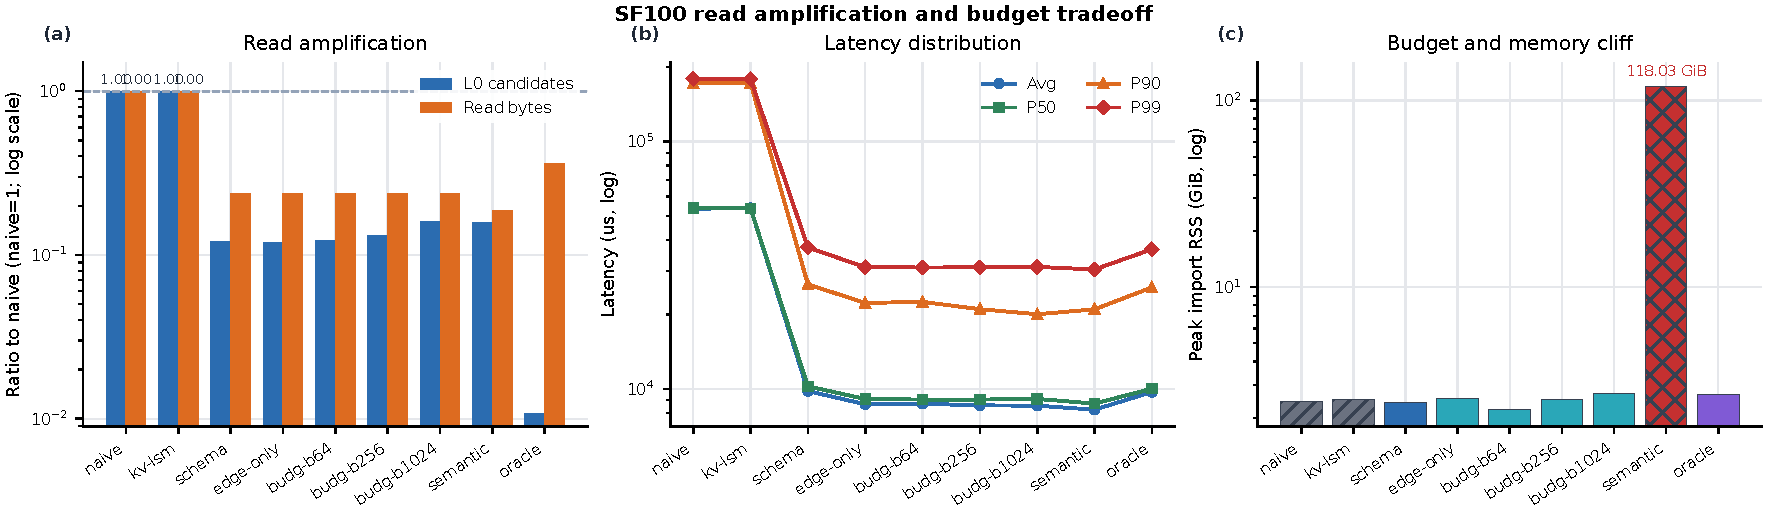
\includegraphics[width=0.98\textwidth]{fig2_sf100_read_budget.pdf}
  \caption{W6 SF100. Panel (a) divides each metric by the naive value and uses
  a logarithmic axis; candidate L0 is primary, while read bytes are secondary
  because offset-array/cache over-read produces high variance. Panel (b) is a
  workload-specific latency distribution; the budget-64 versus schema latency
  gate is \textsc{fallback}. Panel (c) exposes the full-semantic memory cliff.}
  \label{fig:sf100}
\end{figure*}

Figure~\ref{fig:sf100}(a) shows that semantic metadata changes admission: naive
and kv-lsm each accumulate 49.26M candidate-L0 admissions, versus 5.93M for
schema and 6.02M for budget-64. Read-byte measurements are shown for
completeness but are not a primary claim: the reader may reload whole offset
arrays after metadata-cache misses, and SF100 standard deviations are large.
Panel (b) likewise does not establish a stable budget-64 latency win over
schema; their one-standard-deviation gate is \textsc{fallback}.

Panel (a)'s ``normalized cost (naive=1, log)'' is
$x_v/x_{naive}$ for each metric $x$ and variant $v$, displayed on a logarithmic
axis so the candidate, byte, and file ratios remain visible together. It is
not a weighted composite score. Schema cuts candidate admission to 12.0\% of
naive; budget-64 is 12.2\%. Full semantic admits 7.78M candidates because
finer files improve some dimensions while increasing the number of files that
can overlap a source range. Oracle's exact in-memory L0 index admits only
0.53M candidates, but it is an upper-bound reference built after import, not a
durable layout with comparable construction cost. These rows show why file
count and metadata precision must be interpreted jointly.

The main budget result is the resource bound. Table~\ref{tab:variants} shows
that at SF10 budget-64 stays at 13.3~GiB and 2.26~GiB RSS, while full semantic
grows to 14.6~GiB and 8.38~GiB RSS. At SF100, full semantic reaches
118.03~GiB versus 2.21~GiB for budget-64. Schema is a strong static baseline;
budgeted control adds a resource ceiling and a way to redirect precision. In a
real-SF30-derived W7 workload shift, feedback-only control selected a hot
partition in both phases and moved the selected range after the hot range
changed. This is derived workload evidence, not a production trace, but it
tests the mechanism that static schema lacks.

Budget-64 should therefore not be presented as a universal replacement for
schema. On this read matrix its candidate count is slightly higher and its
latency confidence gate does not separate the two. Its additional value is a
hard accounting boundary around degree precision and an input for workload
adaptation. Full semantic demonstrates the opposite endpoint: more metadata
can reduce selected read bytes on this workload, yet its file and import-memory
cost becomes unacceptable at SF100. The meaningful comparison is the
resource/performance envelope, not a claim that one b64 point dominates every
static layout.

\subsection{Compaction retention}

\begin{figure*}[t]
  \centering
  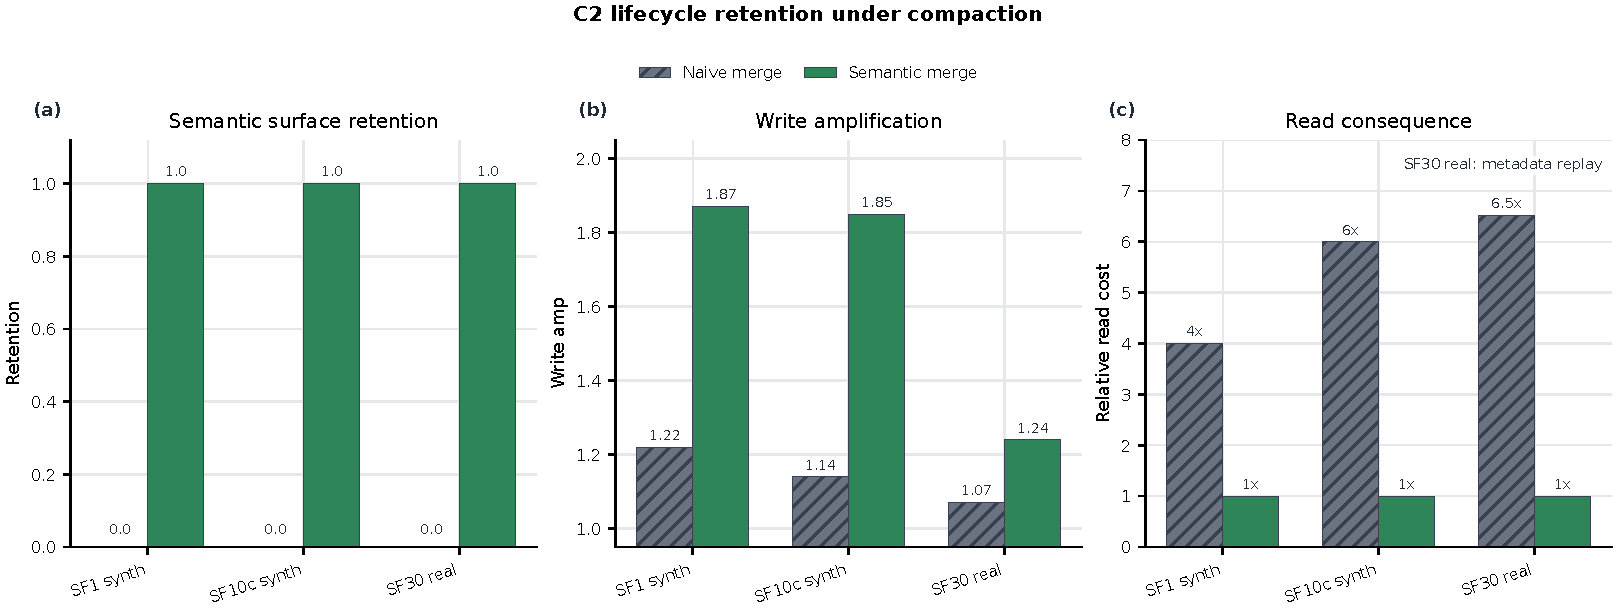
\includegraphics[width=0.98\textwidth]{fig3_c2_lifecycle_retention.pdf}
  \caption{C2 compaction evidence. (a) retention is exact-surface ratio after
  divided by before. (b) write amplification is output bytes divided by logical
  update bytes. (c) is aggregate candidate bytes after merge divided by exact
  partition bytes before; SF30 is metadata replay, not body-read execution.}
  \label{fig:c2}
\end{figure*}

For C2, the exact-surface ratio is the number of edges in topology-exact
segments divided by all edges covered by the merge. Retention divides that
ratio after by before. The controlled synthetic inputs deliberately construct
four and six exact source-label/edge-type partitions; this isolates
merge policy as the causal variable. Naive merge collapses each set to mixed
output and retention 0, producing 4x/6x full-read amplification. Semantic merge
keeps retention 1 and read cost 1x, with write amplification 1.87/1.85 versus
1.22/1.14 for naive.

More formally, for the logical edge multiset $D$ covered by a merge, let
$E(M)$ be edges residing in topology-exact segments under metadata state $M$.
The three reported quantities are

\begin{equation}
\mathrm{ret}=\frac{|E(M_{after})|/|D|}{|E(M_{before})|/|D|},\quad
\mathrm{WA}=\frac{\mathrm{output\ bytes}}{\mathrm{logical\ update\ bytes}},
\label{eq:c2}
\end{equation}

and the read-consequence proxy is aggregate bytes admitted by post-merge
metadata divided by bytes in each queried exact partition before merge. The
denominator is the body that an ideal retained partition would expose, not the
whole database. ``Post-merge metadata'' means that each source-label/edge-type
signature is tested against output headers with the same admission contract as
Equation~\ref{eq:admit}. It does not mean the output bodies were decoded.

Synthetic data is appropriate for the first two rows because it controls the
number and size of exact partitions while keeping logical contents fixed. A
naive output must then admit all four or six equal partitions, making the
4x/6x consequence directly attributable to merge policy rather than LDBC
skew. The real SF30 row supplies external validity using the partitions that
the loader and manifest actually produced.

The real SF30 run processes all 1.09 billion directed edges. Draining L0
produces the 40 observed source-label/edge-type groups and 528 exact L1
segments; 40 is therefore data-derived, not an arbitrary query count. Naive
L1-to-L2 merge yields retention 0 and write amplification 1.07, while semantic
merge yields retention 1 and 1.24. Panel (c) replays those 40 signatures over
post-merge metadata. Naive merge admits 282.16~GB against 43.25~GB of exact
partition bytes, or 6.52x. Semantic merge admits 43.25~GB, or 1.00x. This replay
performs no body decode and supports no SF30 latency claim.

\subsection{Lifecycle coverage and correctness}

The evidence is decomposed by stage. W6 measures flush layout, admission, and
resources; C2 isolates compaction retention and rewrite cost. W7 uses a store
derived from real SF30 CSV, with two phases of eight flushes, 64 hot sources,
and eight queries per source. Feedback-only and static-budgeted policies both
compact the hot range after the first flush of each phase; feedback-only moves
to the new range in phase B, whereas no-feedback performs no hot compaction.
For the last flush, candidate segments per query fall from 2 to 0 and body
reads from 3 to 1 after the selected compaction. This is a controlled
workload-shift mechanism test, not a full SF30 production trace and not evidence
that the flush budget alone predicts future demand.

W9 runs 30 minutes of mixed reads/writes over SF30 starting stores and records
six checkpoints. At the last checkpoint, the measured p99 is 8,740.2~$\mu$s
for schema and 1,274.0~$\mu$s for semantic, with about 163 queries/s and zero
writer errors. However, rewrite bytes are zero for every variant. The trend is
therefore evidence for continued flush, L0 accumulation, and preservation of
the starting layout; it does not execute concurrent semantic compaction and
cannot validate the complete lifecycle.

W13 is a bounded ten-test suite. It checks mixed schema epochs across
compaction/reopen, property deltas at snapshots, old-segment readability,
catalog persistence, reporting boundaries, fixed-width property encoding
changes, edge-label aliases, row encoding epochs, dropped-property behavior,
and exact-versus-mixed pruning after a new edge label. All ten tests pass.
These are implementation correctness tests, not a general online schema
migration benchmark. Together, the stages support a lifecycle-oriented design
without pretending that one run exercised the lifecycle end to end.

The measured/proxy boundary is consequently explicit. W6, W7, W9, and W13
execute their respective prototype paths; controlled C2 executes merge and
read consequences; real-SF30 C2 executes merge but replays only metadata for
the read consequence. SF100 read bytes are measured yet secondary because of
known reader over-read. Every principal number in the paper comes from a
completed artifact, but completion does not make scopes interchangeable.

\section{Related Work}

Dynamic graph stores explore transactional adjacency scans and multiversion
structures \cite{livegraph,teseo}. GraphOne and a recent DGS study examine
mutable graph representations and their tradeoffs \cite{graphone,revisitingdgs}.
LSMGraph combines dynamic updates with multi-level CSR \cite{lsmgraph}; \sys
focuses on semantic evidence used by both read admission and physical rewrite.
These systems establish that update path, versioning, and adjacency layout
matter for evolving graphs. They do not make the same claim that a
property-graph access signature should be persisted as a proof object and
retained across LSM rewrites. Our external artifact runs several systems only
through a common typed-neighbor correctness gate; differing loaders, APIs, and
operation counts prevent an end-to-end speed ranking.

BACH already uses workload and degree distribution to tune LSM-based graph
format and merge choices \cite{bach}. ArceKV adapts generic LSM compaction to
changing key-value workloads \cite{arcekv}. \sys is therefore not claiming the
first workload-aware merge scheduler. Its distinction is the object being
preserved: property-graph semantic evidence, a safe proof rule for skipping,
and measured semantic-surface retention across compaction. Functional storage
decomposition motivates separating access needs from a fixed format
\cite{functionalstorage}. Graph-oriented columnar layouts make a related case
for graph-specific physical organization \cite{columnargraph}.

Traditional LSM filters and range metadata also reject irrelevant files, but
their evidence is normally expressed over keys or membership. SemL0's
dimensions include graph labels, typed relationships, direction, local degree
bounds, and property presence, and their interpretation can depend on a schema
catalog. The novelty is not that summaries can prune; it is that summary
completeness is part of the storage contract, budget selection starts from a
schema-aware baseline, and compaction is measured by whether it retains the
future proof surface. This positioning is narrower than a new graph query
engine and broader than an L0-only filter.

\section{Limitations and Conclusion}

\sys is a prototype, not a complete property-query engine or production graph
database. Property values beyond presence remain prototype-only. SF100 read
bytes carry a reader-over-read caveat, SF100 latency does not pass the
budget-64/schema separation gate, W7 is real-data-derived rather than a trace,
and SF30 C2 read consequence is a metadata proxy. Schema/snapshot evidence is a
bounded correctness suite, not general online migration.

The current budget also optimizes an estimated file unit, not CPU time,
long-term write amplification, or a multi-tenant objective. Its weights are
configured constants plus local feedback, and Low/Medium/High thresholds are
fixed rather than learned. A production controller would need decay, admission
hysteresis, background-I/O limits, and coordination between flush precision
and level compaction. Rich property predicates would additionally require
value summaries whose exactness survives encoding changes. These extensions
fit the same proof rule but are not evaluated here.

The design applies most directly to selective typed-neighbor workloads over
immutable graph segments. A scan that requests every edge type gains little
from semantic partitioning; a workload dominated by high-degree hubs may pay
more file and merge cost; and a store whose schema already creates one physical
relation per edge type may need only the retention contract. Budgeted control
is useful precisely when workload selectivity and materialization cost are
both non-uniform.

Within those boundaries, the result is consistent: graph query semantics can
be persistent storage evidence; every skip must follow an exactness contract;
the evidence needs a file/resource budget; and compaction must explicitly
retain or demote it. Treating compaction as semantic rewrite is the central
systems lesson.

\begin{thebibliography}{99}

\bibitem{lsm}
P. O'Neil, E. Cheng, D. Gawlick, and E. O'Neil.
\newblock The log-structured merge-tree.
\newblock \emph{Acta Informatica}, 33(4):351--385, 1996.

\bibitem{ldbc}
O. Erling et al.
\newblock The LDBC social network benchmark: Interactive workload.
\newblock In \emph{SIGMOD}, 2015.

\bibitem{lsmgraph}
S. Yu et al.
\newblock LSMGraph: A high-performance dynamic graph storage system with
multi-level CSR.
\newblock \emph{Proc. ACM Manag. Data}, 2(6), Article 243, 2024.

\bibitem{livegraph}
X. Zhu et al.
\newblock LiveGraph: A transactional graph storage system with purely
sequential adjacency list scans.
\newblock \emph{PVLDB}, 13(7):1020--1034, 2020.

\bibitem{teseo}
D. De Leo and P. Boncz.
\newblock Teseo and the analysis of structural dynamic graphs.
\newblock \emph{PVLDB}, 14(6):1053--1066, 2021.

\bibitem{graphone}
P. Kumar and H. H. Huang.
\newblock GraphOne: A data store for real-time analytics on evolving graphs.
\newblock In \emph{FAST}, 2019.

\bibitem{revisitingdgs}
J. Su et al.
\newblock Revisiting the design of in-memory dynamic graph storage.
\newblock \emph{Proc. ACM Manag. Data}, 3(1), Article 70, 2025.
\newblock DOI: 10.1145/3709720.

\bibitem{bach}
J. Huang, Y. Cao, S. Ren, B. Wu, and D. Miao.
\newblock BACH: Bridging adjacency list and CSR format using LSM-trees for
HGTAP workloads.
\newblock \emph{PVLDB}, 18(5):1509--1521, 2025.

\bibitem{arcekv}
J. Liu, H. Xie, and S. Luo.
\newblock ArceKV: Towards workload-driven LSM-compactions for key-value store
under dynamic workloads.
\newblock \emph{PVLDB}, 19(5):958--972, 2026.

\bibitem{functionalstorage}
M. Prammer et al.
\newblock Towards functional decomposition of storage formats.
\newblock In \emph{CIDR}, 2025.

\bibitem{columnargraph}
P. Gupta, A. Mhedhbi, and S. Salihoglu.
\newblock Columnar storage and list-based processing for graph database
management systems.
\newblock \emph{PVLDB}, 14(11):2491--2504, 2021.

\end{thebibliography}

\end{document}
